\documentclass[12pt,letterpaper]{report}
\usepackage[letterpaper,left=1.2in,right=1.2in,top=1in,bottom=1in]{geometry}
\usepackage{setspace,epsfig,rawfonts,graphicx,graphicx,epsf,psfrag}
\usepackage{amssymb,amsfonts,amsmath,amsthm}
\usepackage{mathtools}
\usepackage[noadjust]{cite}
\usepackage{appendix}
%\usepackage[cmex10]{amsmath}
\usepackage{array}
%\usepackage{mdwmath}
%\usepackage{mdwtab}
\usepackage{eqparbox}
%\usepackage{amsthm}
%\usepackage[tight,footnotesize]{subfigure}
%\usepackage[caption=false,font=footnotesize]{subfig}
\usepackage{multirow}
\usepackage{chngcntr}
\usepackage{etoolbox}
\usepackage[chapter]{algorithm}
%\part{title}\usepackage{algorithmic}
\usepackage{bm}

\usepackage{float,textcomp}
\usepackage{indentfirst}
\usepackage{times}
\usepackage{psfrag}
\usepackage{graphicx}
\usepackage{epstopdf}


\usepackage{algorithm}
\usepackage{color}
\usepackage[font=small]{caption}
\usepackage{subcaption}
\usepackage{algpseudocode}
\usepackage{textcomp}
\usepackage{booktabs}
\usepackage{lipsum}
\usepackage{cancel} % for cancelto method

\usepackage[linktocpage,bookmarksopen,bookmarksnumbered]{hyperref}

\usepackage{pdfpages}

%\usepackage[nottoc,numbib]{tocbibind}
 %\usepackage[pdftex]{graphicx}
 
\newcommand{\nn}{\nonumber}
\newcommand{\var}{\sigma^2}
\newcommand{\Rho}{\mathrm{P}}
\newcommand{\Tr}{\mathrm{Tr}} 
\newcommand{\diag}{\mathrm{diag}} 
%\DeclareMathOperator{\Tr}{Tr}
% \newcommand{\E}{\mathrm{E}}
\newcommand{\Prob}{\mathrm{Pr}}
% Theorems
\newtheorem{myth}{Theorem}
\newtheorem{mypro}{Proposition}
\newtheorem{mylem}{Lemma}
\newtheorem{mycor}{Corollary}
% Sets
\newcommand{\R}{\mathbb R}
% \newcommand{\I}{\mathbb I}
\newcommand{\C}{\mathbb C}
\newcommand{\Z}{\mathbb Z}
\newcommand{\BBE}{\mathbb E}
% Vectors
\newcommand{\av}{{\bf a}}
\newcommand{\bv}{{\bf b}}
\newcommand{\cv}{{\bf c}}
\newcommand{\dv}{{\bf d}}
\newcommand{\ev}{{\bf e}}
\newcommand{\fv}{{\bf f}}
\newcommand{\gv}{{\bf g}}
\newcommand{\hv}{{\bf h}}
\newcommand{\iv}{{\bf i}}
\newcommand{\jv}{{\bf j}}
\newcommand{\kv}{{\bf k}}
\newcommand{\lv}{{\bf l}}
\newcommand{\mv}{{\bf m}}
\newcommand{\nv}{{\bf n}}
\newcommand{\ov}{{\bf o}}
\newcommand{\pv}{{\bf p}}
\newcommand{\qv}{{\bf q}}
\newcommand{\rv}{{\bf r}}
\newcommand{\sv}{{\bf s}}
\newcommand{\tv}{{\bf t}}
\newcommand{\uv}{{\bf u}}
\newcommand{\wv}{{\bf w}}
\newcommand{\vv}{{\bf v}}
\newcommand{\xv}{{\bf x}}
\newcommand{\yv}{{\bf y}}
\newcommand{\zv}{{\bf z}}
\newcommand{\zerov}{{\bf 0}}
\newcommand{\onev}{{\bf 1}}
% Matrices
\newcommand{\Am}{{\bf A}}
\newcommand{\Bm}{{\bf B}}
\newcommand{\Cm}{{\bf C}}
\newcommand{\Dm}{{\bf D}}
\newcommand{\Em}{{\bf E}}
\newcommand{\Fm}{{\bf F}}
\newcommand{\Gm}{{\bf G}}
\newcommand{\Hm}{{\bf H}}
\newcommand{\Id}{{\bf I}}
\newcommand{\Jm}{{\bf J}}
\newcommand{\Km}{{\bf K}}
\newcommand{\Lm}{{\bf L}}
\newcommand{\Mm}{{\bf M}}
\newcommand{\Nm}{{\bf N}}
\newcommand{\Om}{{\bf O}}
\newcommand{\Pm}{{\bf P}}
\newcommand{\Qm}{{\bf Q}}
\newcommand{\Rm}{{\bf R}}
\newcommand{\Sm}{{\bf S}}
\newcommand{\Tm}{{\bf T}}
\newcommand{\Um}{{\bf U}}
\newcommand{\Wm}{{\bf W}}
\newcommand{\Vm}{{\bf V}}
\newcommand{\Xm}{{\bf X}}
\newcommand{\Ym}{{\bf Y}}
\newcommand{\Zm}{{\bf Z}}
% Calligraphic
\newcommand{\Ac}{{\cal A}}
\newcommand{\Bc}{{\cal B}}
\newcommand{\Cc}{{\cal C}}
\newcommand{\Dc}{{\cal D}}
\newcommand{\Ec}{{\cal E}}
\newcommand{\Fc}{{\cal F}}
\newcommand{\Gc}{{\cal G}}
\newcommand{\Hc}{{\cal H}}
\newcommand{\Ic}{{\cal I}}
\newcommand{\Jc}{{\cal J}}
\newcommand{\Kc}{{\cal K}}
\newcommand{\Lc}{{\cal L}}
\newcommand{\Mc}{{\cal M}}
\newcommand{\Nc}{{\cal N}}
\newcommand{\Oc}{{\cal O}}
\newcommand{\Pc}{{\cal P}}
\newcommand{\Qc}{{\cal Q}}
\newcommand{\Rc}{{\cal R}}
\newcommand{\Sc}{{\cal S}}
\newcommand{\Tc}{{\cal T}}
\newcommand{\Uc}{{\cal U}}
\newcommand{\Wc}{{\cal W}}
\newcommand{\Vc}{{\cal V}}
\newcommand{\Xc}{{\cal X}}
\newcommand{\Yc}{{\cal Y}}
\newcommand{\Zc}{{\cal Z}}


\def\E{\textrm{E}}

\newcommand{\boldeta}{\boldsymbol{\eta}}
%\input macros
\newcommand*{\MyScale}{0.85}

%\newtheorem{example}{Example}[chapter]
%\theoremstyle{definition}
%\newtheorem{assumption}{Assumption}[chapter]

\renewcommand{\bibname}{References}
\newcommand{\mf}[1]{\mathbf{#1}}
\newcommand{\bfb}{\mathbf{b}}
\newcommand{\bfu}{\mathbf{u}}
\renewcommand{\Re}{\mbox{Re}}
\renewcommand{\Im}{\mbox{Im}}

%\newcommand{\lemmaref}[1]{Lemma \ref{#1}}
%\newcommand{\tr}{{\rm tr}}
%\newcommand{\diff}{{\rm d}}
%\newtheorem{theorem}{Theorem}
%\newtheorem{lemma}{Lemma}
%\newtheorem{property}{Property}
%\newtheorem{proposition}{Proposition}
%\newtheorem{definition}{Definition}
%\numberwithin{theorem}{chapter} % important bit
%\numberwithin{lemma}{chapter} % important bit
%\numberwithin{proposition}{chapter} % important bit

\def\ie{{\it i.e.,\ \/}}
\def\defeq{{\stackrel{\Delta}{=}}}
\def\mbbE{\mathbb{E}}
\newcommand{\state}{(\mathbf{e},\mathbf{w})}
\newcommand{\sst}{\mathcal{S}\backslash\mathcal{S}_t}
\newcommand{\eu}{\mathcal{S}\backslash\{t\}\backslash \mathcal{U}}
\def\scalefig#1{\epsfxsize #1\textwidth}
\def\nn{{\nonumber}}

\newcommand{\tabincell}[2]{\begin{tabular}{@{}#1@{}}#2\end{tabular}}
\newsavebox{\tablebox}



\AtBeginEnvironment{subappendices}{%
\chapter*{Appendix}
\addcontentsline{toc}{chapter}{Appendices}
\counterwithin{figure}{chapter}
\counterwithin{table}{chapter}
}



% math operators and functions
\DeclareMathOperator*{\argmin}{arg\,min}
\DeclareMathOperator*{\argmax}{arg\,max}
%\DeclareMathOperator*{\diag}{diag}
\DeclareMathOperator*{\Diag}{Diag}
\DeclareMathOperator*{\ddiag}{ddiag}
%\newcommand{\Tr}{\mathrm{Tr}}
\newcommand{\grad}{\mathrm{grad}}
\newcommand{\Hess}{\mathrm{Hess}}
\newcommand{\dist}{\mathrm{dist}}
\newcommand{\e}[1]{\mathrm{e}^{#1}}
\renewcommand{\qedsymbol}{$\blacksquare$}
% real, imag, transpose, conj transpose
\newcommand{\herm}{^{\mathsf{H}}}
\newcommand{\T}{^{\mathsf{T}}}
\newcommand{\re}{\mathrm{Re}}
\newcommand{\im}{\mathrm{Im}}
% sets
%\newcommand{\C}{\mathbb{C}}
\newcommand{\CM}{\mathbb{C}^M}
\newcommand{\CML}{\mathbb{C}^{M\times L}}
\newcommand{\CLJ}{\mathbb{C}^{L\times J}}
\newcommand{\Uj}{\mathcal{U}(1)^{\times J}}
\newcommand{\St}[2]{{\rm ST}_{\bm{B}}(#1\times #2)}
\newcommand{\StB}[2]{{\rm ST}_{\bm{B}}(#1\times #2)}
\newcommand{\StL}[2]{{\rm ST}_{\bm{\Lambda}}(#1\times #2)}
% common vectors
\newcommand{\w}{\bm{w}}
\newcommand{\W}{\bm{W}}
\newcommand{\z}{\bm{z}}
\newcommand{\xk}{\bm{x}_k}
\newcommand{\Xk}{\bm{X}_k}
\newcommand{\bb}{\bm{b}}
\newcommand{\uu}{\bm{u}}
%common riemannian vectors
\newcommand{\etaw}{\bm{\eta}_{\w}}
\newcommand{\etawt}{\bm{\eta}_{\w_t}}
\newcommand{\etawj}{\bm{\eta}_{\w_j}}
\newcommand{\etawjj}{\bm{\eta}_{\w_{j_1}}}
\newcommand{\etab}{\bm{\eta}_{\bb}}
\newcommand{\uw}{\uu_{\w}}
%\newcommand{\vv}{\bm{v}}
%\newcommand{\uv}{\bm{u}_{\vv}}

\newcommand{\SINR}{\mathrm{SINR}}
\newcommand{\MAC}{\mathrm{MAC}}
\newcommand{\BC}{\mathrm{BC}}




\newcommand{\beq}{\begin{equation}}
\newcommand{\eeq}{\end{equation}}
\newcommand{\bsubeq}{\begin{subequations}}
\newcommand{\esubeq}{\end{subequations}}
\newcommand{\barp}{\bar z}
\newcommand{\Pb}{\mbox{P}}


\newtheorem{proposition}{Proposition}
\newtheorem{observation}{Observation}
\newtheoremstyle{mystyle}%                % Name
{}%                                     % Space above
{}%                                     % Space below
{\itshape}%                             % Body font
{}%                                     % Indent amount
{}%                            % Theorem head font
{.}%                                    % Punctuation after theorem head
{ }%                                    % Space after theorem head, ' ', or \newline
{{\bfseries \thmname{#1}\thmnumber{ #2}} (\thmnote{#3})}%                                     % Theorem head spec (can be left empty, meaning `normal')
%\thmname{#1}\thmnumber{ #2}:\thmnote{ #3}

\newtheoremstyle{mystyle2}%                % Name
{}%                                     % Space above
{}%                                     % Space below
{\itshape}%                             % Body font
{}%                                     % Indent amount
{}%                            % Theorem head font
{.}%                                    % Punctuation after theorem head
{ }%                                    % Space after theorem head, ' ', or \newline
{{\bfseries \thmname{#1}\thmnumber{ #2}}}%   

\theoremstyle{mystyle}
\newtheorem{thm}{Theorem}
\newtheorem{lem}[thm]{Lemma}
\newtheorem{prop}[thm]{Proposition}
\newtheorem{cond}[thm]{Condition}
\newtheorem{defn}[thm]{Definition}


\theoremstyle{mystyle2}
\newtheorem{thm2}{Theorem}
\newtheorem{cor}[thm]{Corollary}
\newtheorem{conj}[thm]{Conjecture}
\newtheorem{exmp}[thm]{Example}

\theoremstyle{remark}
\newtheorem*{rem}{Remark}
\newtheorem*{note}{Note}


%\newtheorem{theorem}{Theorem}
%\newtheorem{lemma}[theorem]{Lemma}
%\newtheorem{definition}{Definition}
%\newtheorem{prop}{Proposition}
\newcommand{\zding}[1]{\textcolor{red}{/*Prof. Ding: #1*/}}
\newcommand{\mdr}[1]{\textcolor{red}{/*Mason: #1*/}}

\definecolor{darkgreen}{rgb}{0.0, 0.5, 0.0}

\captionsetup[figure]{font=small}
\captionsetup[table]{font=small}
\graphicspath{{./images/}}

\begin{document}

\doublespacing
\renewcommand{\labelenumi}{(\arabic{enumi})}

% the official guidance on the UCD title page is from here:
% sample: https://ucdavis.app.box.com/v/GSSampleTitlePage
% template: https://ucdavis.app.box.com/v/TitlePageTemplate
\includepdf{title_page/title_page_mdr.pdf} % include UCD template title page in frontmatter

\pagenumbering{roman}

\stepcounter{page} % increment page number, accounting for title page
\chapter*{Acknowledgements}
% \thispagestyle{empty}

Completing this dissertation would not have been possible without the support of many kind, driven, and supportive researchers. My advisor, Zhi Ding, who secured the funding for my degree\footnote{The research conducted in this dissertation was supported by the National Science Foundation under the following grants: ECCS-1711823, ECCS-2029027, and CNS-2002937.} and who always challenged me to be a better researcher. Lifeng Lai and Khaled Abdel-Ghaffar, who served on both my qualifying exam and dissertation committees. Daniela Cabric and Zhaojun Bai, who graciously served as members of my qualifying exam committee. My lab mates and collaborators, particularly Zhenyu Liu, Yu-Chien Lin, Carlos Feres, Siyu Qi, and Lahiru Chamain.

Outside of my advisors and colleagues in research, I had numerous other mentors and collaborators during my time at UC Davis. Hooman Rashtian, with whom I taught as a teaching assistant for several undergraduate courses and the COSMOS program. My colleagues in 2021-22 cohort of the Professors for the Future Fellowship as well as the organizers of the program, Teresa Dillinger, Ellen Hartigan-O'Connor, and David Blancha. My colleagues and consultees from the Graduate Writing Fellows program, and the head of the program, and Katherine Gossett.

Finally, my family and friends who have tirelessly supported me on my doctoral journey. My parents, Michael and Gail, who have always provided me with opportunities to succeed. My brother, Zachary, who inspired me to embark on this doctoral journey, who always advocated for me, offered me advice, and continues to inspire me to this day. My friends from Olin College, Ankur, Carly, Brandon, Abe, and Wanyi (an honorary Oliner). My best friend from Carnegie Mellon, Josh Choi. My friends from Temple University Japan, Ty Givens and Casey Farrington. Most importantly, my partner, Misha Nguyen, who keeps me grounded and who fills my life with love and light.

% \clearpage

\tableofcontents
\listoffigures
\listoftables

\newpage
\pagenumbering{arabic}
\newpage
% {\baselineskip 14pt \rightline{Mason del Rosario} \rightline{September,
% \the\year} \rightline{Electrical and Computer Engineering}} \vspace{27pt}
\chapter*{\centering Abstract}
\addcontentsline{toc}{chapter}{Abstract}

Future wireless communications networks will implement massive MIMO technologies to significantly improve spectrum efficiency where a base station (BS) with large multiantenna arrays serve a large number of user equipment (UE) terminals. Such multiantenna arrays enable high capacity communications via beamforming, as evidenced by work in information theory. To achieve the expected capacity in massive MIMO networks, the base station requires accurate estimates of downlink channel state information (CSI) at the transmitter for precoding.

Typically, receivers can estimate CSI using known pilot signals. In the special case of time-division duplex (TDD) mode, channel reciprocity allows the BS to estimate the downlink CSI via pilots in uplink transmissions. However, in frequency division duplex (FDD) mode, channel reciprocity between uplink and downlink channels is comparatively weak, and the BS must also rely on feedback from the UE to estimate downlink CSI. Specifying an appropriate CSI feedback scheme is a key issue and involves reducing feedback bandwidth while maintaining accurate downlink CSI estimates.

Conventional methods for CSI feedback compression can rely on compressive sensing (CS), which seeks to reconstruct high-dimensional data based on low-dimensional measurements. Many CS methods are based on convex relaxations of an underdetermined least-squares problem, and such methods rely on iterative solvers (e.g., the proximal gradient method). When using an iterative solver, reconstruction can consume an undue amount of time even when measurements are available, making faster CSI reconstruction methods an attractive research direction.

Recent works in deep learning for compressed CSI estimation have presented viable alternatives to CS methods. These proposed methods typically employ convolutional neural networks (CNNs) to extract compressed representations of high-dimensional CSI. Deep learning architectures used in CNN-based works can be placed in one of two categories. The first category is CNN-based autoencoders, networks which utilize two subnetworks: an encoder network which learns a low-dimensional representation with the original data as an input and a decoder network which estimates the original data with the encoder's low-dimensional representation as an input. The second category is unrolled optimization networks, inspired by the aforementioned CS methods by structuring the CNN as a finite number of repeated blocks with each block imitating an iteration of a given CS algorithm.

This dissertation explores both CNN autoencoders and unrolled optimization networks for CSI estimation. However, instead of taking a black box approach, we focus on domain knowledge, including physical insight into the wireless channel or features of the communications protocol, to improve the performance of these CSI estimation networks with respect to accuracy, feedback rate, or network efficiency. Prior works have demonstrated superior performance of these architectures over conventional CS methods, and this dissertation investigates the myriad ways that domain knowledge of wireless channels and communications protocols can be leveraged to improve CSI estimation.

The first research direction discussed is spherical normalization, which involves scaling CSI data by the channel's power and can improve CSI estimation accuracy without increasing model complexity. The second research innovation applies deep differential encoding, which estimates the error in CSI estimates based on a one-step Markov model. We describe a deep differential encoder which offers a significant reduction in computational complexity when compared to state-of-the-art recurrent neural networks while achieving superior estimation accuracy. In the third research direction, we use the practical, sparse frequency domain pilots to estimate the truncated delay domain, enabling the usage of the delay domain CSI commonly adopted in deep learning based CSI estimation works. Additionally, we implement a heterogeneous differential encoder, which uses different network architectures at each timeslot and offers superior estimation accuracy over the prior homogeneous differential encoders. In the final chapter, we propose model reuse, where a smaller model is used multiple times on a relatively large input, and we show that this method can maintain comparable estimation accuracy while reducing computational complexity.
\chapter{Introduction}
\label{chap:intro}

% TODO: updates to make:
% - 1.1 MIMO Channel overview
% 	- Add more discussion about MIMO CSI, capacity, precoding/beamforming, 
%	- Add details about 3GPP specificaions (possibly from latest preprint?)
% - Add more 

% Section \ref{sect:notation} introduces the notation used through this work.
This dissertation details work in improving the accuracy and efficiency of deep learning methods for MIMO channel state information estimation. This chapter provides the necessary background to understand the contributions of the dissertation. Section \ref{sect:mimo_model} provides an overview of the MIMO channel and the importance of CSI estimation in MIMO-based communications networks. Section \ref{sect:channel_model} discusses MIMO channel models and introduces the primary channel model used in this work, the COST2100 model. Section \ref{sect:classic_estimation} discusses prior work in compressed sensing for CSI estimation. Section \ref{sect:dl_overview} provides a generic overview of deep learning. 
Boldface lowercase (uppercase) letters indicate vectors (matrices). Unless otherwise specified, the norm $\|\cdot\|$ indicates the Frobenius norm. Superscripts $^T$ ($^H$) indicate the transpose (Hermitian transpose).
% recent work in deep learning for CSI estimation in MIMO networks

\section{MIMO Channel Overview}
\label{sect:mimo_model}

\begin{figure}[!hbtp]
\centering
{
	\fontsize{6pt}{8pt}
	\def\svgwidth{0.8\columnwidth}
	\input{images/mimo-schematic.pdf_tex}
}
\caption{Example multi-antenna transmitter (BS, gNB) and single-antenna user equipment (UE) and relevant system values.}
\label{fig:mimo_schematic}
\end{figure}

In this work, we consider a MIMO channel with a multiple antennas ($N_B \gg 1$) at the transmitter (gNodeB or gNB) servicing a single user equipment (UE) with a single antenna. Under orthogonal frequency division multiplexing (OFDM) with $N_f$ subcarriers, the received symbols on the $m$-th subcarrier for the downlink and the uplink at the receiver are given as
\begin{align*}
	y_{d,m} &= \mathbf h_{d,m}^H\mathbf w_{t,m}x_{d,m} + n_{d,m}.
	% y_{u,m} &= \mathbf w_{r,m}^H\mathbf h_{u,m}x_{u,m} + \mathbf w_{r,m}^H\mathbf n_{u,m},
\end{align*}
where the individual system values are defined in Table~\ref{tab:mimo-params}, and a representative system model is viewable in Figure~\ref{fig:mimo_schematic}. The resulting downlink and uplink channel state information (CSI) matrices are given as
\begin{align*} 
	\bar{\mathbf H}_d &= \begin{bmatrix} \mathbf h_{d,1} & \dots & \mathbf h_{d,N_f}\end{bmatrix}^H \in \mathbb C^{N_f \times N_b}.
	% \bar{\mathbf H}_u &= \begin{bmatrix} \mathbf h_{u,1} & \dots & \mathbf h_{u,N_f}\end{bmatrix}^H \in \mathbb C^{N_f \times N_b}.
\end{align*}
\begin{table}[]
\renewcommand{\arraystretch}{1.25}
\centering
\caption{MIMO system variables considered in this work.}
\label{tab:mimo-params}
\begin{tabular}{c|c|l}
\toprule
\textbf{Symbol}   	  	  & \textbf{Dimension}            & \textbf{Description} \\ \midrule
$y_{d,m}$ 		  	  	  & $\mathbb{C}^{1}$ 			  & Received downlink symbol on $m$-th subcarrier  \\ \hline
$\mathbf h_{d,m}$ 	  	  & $\mathbb{C}^{N_b \times 1}$   & Downlink channel on $m$-th subcarrier  \\ \hline
$\bar{\mathbf H}_{d}$ 	  & $\mathbb{C}^{N_f \times N_b}$ & Downlink CSI (spatial-frequency domain)  \\ \hline
$\mathbf w_{t,m}$ 	  	  & $\mathbb{C}^{N_b \times 1}$   & Transmitter precoding vector for $m$-th subcarrier  \\ \hline
$x_{d,m}$ 		  	  	  & $\mathbb{C}^{1}$ 			  & Trasmitted symbol on $m$-th subcarrier  \\ \hline
$n_{d,m}$ 		  	  	  & $\mathbb{C}^{1}$ 			  & Downlink noise on $m$-th subcarrier  \\ \hline
$\tilde{\mathbf H}_{d}$   & $\mathbb{C}^{N_f \times N_b}$ & Downlink CSI (angular-delay domain)  \\ \hline
$\mathbf H_{d}$   		  & $\mathbb{C}^{R_d \times N_b}$ & Truncated downlink CSI (angular-delay domain)  \\ \hline
% $y_{u,m}$ 		  & $\mathbb{C}^{1}$ 			  & Received uplink symbol on $m$-th subcarrier  \\ \hline
% $\mathbf h_{u,m}$ & $\mathbb{C}^{N_b \times 1}$   & Uplink channel on $m$-th subcarrier  \\ \hline
% $\mathbf H_{u}$   & $\mathbb{C}^{N_f \times N_b}$ & Downlink impulse response on $m$-th subcarrier  \\ \hline
% $\mathbf w_{r,m}$ & $\mathbb{C}^{N_b \times 1}$   & Received precoding vector for $m$-th subcarrier  \\ \hline
% $x_{u,m}$ 		  & $\mathbb{C}^{1}$ 			  & Received symbol on $m$-th subcarrier  \\ \hline
% $\mathbf n_{u,m}$ & $\mathbb{C}^{1}$ 			  & Uplink noise on $m$-th subcarrier  \\ \hline
\end{tabular}
\end{table}
To achieve near-capacity transmission rates, the transmitter needs access to an appropriate estimate of $\bar{\mathbf H}_d$ \cite{ref:goldsmith2003capacity}. Such estimates enable the use of linear precoding techniques (e.g., conjugate beamforming or zero-forcing beamforming) to realize appreciable spectral and power efficiency gains \cite{ref:yang2013performance}. Downlink CSI estimation can be performed in time division duplex (TDD) by using uplink pilots due to channel reciprocity \cite{ref:Kaltenberger2010relative,ref:mi2017massive,ref:Gao2010utilization}. In contrast, frequency domain duplex (FDD) does not admit channel reciprocity due to frequency-selective channels, meaning CSI estimates must be acquired at the UE using pilot signals, and these estimates must be compressed then fed back to the BS.

\section{Practical Pilot-based Channel Estimation in 4G/5G Networks}
\label{sect:pilots}

% \section{Sparse Pilots in Practical Networks}
To estimate the downlink CSI in wireless networks, transmitters allocate pilot reference signals. To reserve spectral resources, pilots are restricted to a limited number of spatial-frequency positions, and the allocation of these pilots is defined in the 3GPP technical standards, TS 36.211 for 4G/LTE networks \cite{ref:3gpp.36.211} and TS 38.211 for 5G/NR networks \cite{ref:3GPPTS38.211V15.8.0}. In these two standards, the pilots are called CSI reference signals (CSI-RS) or demodulation reference signals (DM-RS), respectively. Figure~\ref{fig:lte-vs-5g} shows valid placements of CSI-RS/DM-RS in the time-frequency resource grid as defined by TS 36.211 and TS 38.211.

\begin{figure}[!hbtp]
    \centering
    \includegraphics[width=\linewidth]{LTE_vs_5GNR_resource_grid.png}
    \caption{(a) LTE resource blocks with CSI-RS locations. (b) 5G NR resource blocks with DM-RS locations.}
    \label{fig:lte-vs-5g}
\end{figure}

While many using deep learning for CSI estimation do not address pilot estimation explicitly, a few works have incorporated pilot estimation into the CSI feedback problem. 

\section{Geometric Stochastic Channel Models (GSCMs)}
\label{sect:channel_model}

Ideally, the datasets used for the CSI estimation task would be derived from measurement campaigns (e.g., see \cite{ref:shepard2016argoschannel,ref:du2021interuserangle,ref:li20222finegrained}). However, the financial and labor costs of acquiring these datasets can be prohibitive in certain situations. In such situations, researchers rely on  rely on geometric stochastic channel models (GSCMs), models which are so called since they consider the \textbf{geometry} of scatterers in the wireless environment and the \textbf{stochastic} nature of the channel. Simulations based on GSCMs are advantageous to researchers for a a few reasons:
\begin{enumerate}
	\item Simulations permit the generation a large quantities of data in a (relatively) short period of time.
	\item Simulations enable the adjustment of parameters of the communications system (e.g., carrier frequency, UE mobility, subcarrier spacing).
\end{enumerate}

GSCMs consider the problem of modeling the wireless channels at two different scales. At a small-scale, the focus is on th meodeling of ``scatterers,'' objects in the environment which reflect the electromagnetic waves transmitted during. Examples of scatterers in an outdoor environment are buildings, balconies, cars, and trees, while examples of scatters in an indoor environment are walls, furniture, and people. Due to the presence of many scatterers, electromagnetic waves transmitted from a BS arrive at UEs along multiple paths at different delays, and accordingly, the scatterers are often referred to as \textbf{multipath components (MPCs)}. From the UE's perspective, the MPCs are often grouped together in specific delay regions, and each such grouping of MPCs is referred to as a \textbf{cluster}. In GSCMs, modeling is done at a cluster-level, capturing the diverse effects of many MPCs that are present in typical real-world wireless channels. Modeled clusters are typically parameterized by three values: delay, direction of departure (DoD), and direction of arrival (DoA).  

While the modeling of MPCs and clusters is vital, also vital is ensuring that the results of the GSCM-based simulations are statistically consistent with the measured channel data. This consistency is ensured by selecting \textbf{large-scale parameters (LSPs)}, examples of which are the delay spread and the angular spread. In designing GSCMs, the goal is to balance the fidelity of cluster behavior (based on delay, DoD, DoA) and of LSPs when compared to measured channel data. In practice, researchers implement GSCMs based on two different modeling approaches: system-level modeling or cluster-level modeling.

In system-level modeling, the interaction(s) between the BS and the UE(s) is first defined by choosing LSPs. This selection of LSPs is done by sampling from probability distributions. Based on the LSPs, the clusters and MPCs for each BS/UE interaction is defined.

While some well-known channel models, such as the 3GPP Spatial Channel Model (SCM) \cite{ref:kyosti2007winner} and the WINNER II \cite{ref:kyosti2007winner}, adopt the system-level approach, this modeling approach has some salient limitations. First, system-level models do not lend themselves well to high-mobility scenarios, as the LSPs are likely to change as the position of UEs change substantially. Second, system-level models make the addition of new LSPs (e.g., inter-link correlation) to a given interaction.

In contrast with system-level models, cluster-level models begin with cluster/MPC definition then move on to LSPs. First, a large number of clusters are defined by sampling from a chosen probability distribution. Then, the location(s) of UE(s) is (are) defined, and the scattering of each cluster is calculated based on the ``visibility'' of UEs with respect to the clusters. Finally, the LSPs are synthesized by sampling from a given probability distribution.

The cluster-level approach addresses both of the issues associated with system-level approaches. Simulating time-varying channels with high mobility is straightforward since it involves recalculating UE visibility and LSPs, and layering new LSPs into the model is simple since it is the last step of the simulation.

For all CSI tests, we mainly rely on a cluster-level GSCM, the COST2100 channel model,  \cite{ref:liu2012cost2100}. We use two datasets with a single base station (gNB) and a single user equipment (UE) in the following scenarios:
\begin{enumerate}
	\item \textbf{Indoor} channels using a 5.3GHz downlink at
	0.001 m/s UE velocity, served by a
	gNB at center of a $20$m$\times 20$m coverage area.
	\item \textbf{Outdoor} channels using a 300MHz downlink at 0.9 m/s UE velocity served by a gNB at center 
	of a $400$m$\times 400$m coverage area.
\end{enumerate}
In both scenarios, we use the parameters listed in Table~\ref{tab:cost-params}.
\begin{table}[]
\centering
\caption{Parameters used for COST2100 simulations for both Indoor and Outdoor datasets.}
\label{tab:cost-params}
\begin{tabular}{c|c|l}
\toprule
\textbf{Symbol} & \textbf{Value} & \textbf{Description} \\ \midrule
$N_b$ 			& 32			 & Number of antennas at gNB  \\ \hline
$N_f$ 			& 1024			 & Number of subcarriers for OFDM link  \\ \hline
$R_d$ 			& 32			 & Number of delay elements kept after truncation  \\ \hline
$N$ 			& $10^6$		 & Total number of samples per dataset  \\ \hline
$T$ 			& 10		 	 & Number of timeslots  \\ \hline
$\delta$		& 40 ms			 & Feedback delay interval between consecutive CSI timeslots  \\ \bottomrule
\end{tabular}
\end{table}

\section{Classical CSI Estimation}
\label{sect:classic_estimation}

Works in compressive feedback for CSI estimation in MIMO networks can be placed in three broad categories. The first category includes works which use direct quantization of continuous CSI elements to discrete levels. The quantized CSI are encoded and fed back to the transmitter \cite{ref:makki2012hybrid,ref:shirani2009channel}. The second category includes works which use compressed sensing, a technique which applies a random measurement matrix at the transmitter and the receiver \cite{ref:rao2014distributed, ref:eltayeb2014compressive}. Compressed sensing assumes matrices to be encoded and fed back meet certain sparsity requirements, and compressed sensing algorithms require iterative solvers \cite{ref:do2008sparsity} for decoding, resulting in undesired latency.

The last category of work in compressive CSI feedback uses deep learning (DL), neural networks with numerous layers which are trained on large datasets using backpropagation. We will provide the background knowledge needed for deep learning in Chapter 2, Section~\ref{sect:dl_overview}.

\section{Objective and Contributions}

Successful efforts in DL for CSI estimation have typically utilized convolutional neural networks (CNNs) in an autoencoder structure \cite{ref:csinet}. Variations on the CNN-based autoencoder have investigated different network architectures \cite{ref:Lu2020CRNet}, variational training frameworks \cite{ref:Hussien2020PRVNet}, and denoising modules \cite{ref:Sun2020AnciNet}. These architectural changes are largely inspired by successful application of DL in image compression \cite{ref:szegedy2017inception,ref:balle2017end,ref:xie2012image}.

While they can continue to push the state-of-the-art in CSI reconstruction accuracy, architectural optimizations may ultimately follow the same trends of fields such as language modeling, where state-of-the-art performance requires prohibitively massive compute \cite{ref:brown2020language}. In this proposal, we take a different approach seek to improving compressive channel feedback by focusing on domain knowledge and physical insight.
% While the powerful functional approximation of deep CNNs has enabled state-of-the-art CSI reconstruction accuracy, they run the risk falling into the same trap as the image.

This thesis details our attempts to use domain knowledge to enhance the performance and the efficiency of neural networks for CSI estimation (for a visual summary, see Figure~\ref{fig:contrib}). Section~\ref{chap:sph_norm} details our work in power-based normalization, which leverages CSI sparsity. Section ~\ref{chap:markovnet} describes our work in differential encoding, which exploits temporal coherence of CSI. Section~\ref{chap:p2d} describes our work in pilot-based delay domain CSI estimation.

\begin{figure}[htb] \centering 
	{
	  \fontsize{4pt}{4pt}
	  \def\svgwidth{0.9\columnwidth}
	  % \input{images/cnns-venn-diagram-contrib.pdf_tex}
	}
	\caption{Venn diagram highlighting different aspects of domain knowledge in CNN-based CSI compressive feedback, relevant convolutional networks, and our contributions.}
	\label{fig:contrib}
\end{figure}
\input{./source_file/Thesis_Chap2.tex}
\input{./source_file/Thesis_Chap3.tex}
\chapter{Spectrum-efficient Pilot-based CSI Feedback}
\label{chap:p2d}

This chapter details a scheme for acquiring angular-delay domain CSI at the UE based on a limited number of spatial-frequency domain pilots. This scheme adheres to the 3GPP standard for pilot allocation across time-frequency resources.

\section{Sparse Pilots in Practical Networks}

To estimate the downlink CSI in wireless networks, transmitters allocate pilot reference signals. To reserve spectral resources, pilots are restricted to a limited number of spatial-frequency positions, and the allocation of these pilots is defined in the 3GPP technical standards, TS 36.211 for 4G/LTE networks \cite{ref:3gpp.36.211} and TS 38.211 for 5G/NR networks \cite{ref:3GPPTS38.211V15.8.0}. In these two standards, the pilots are called CSI reference signals (CSI-RS) or demodulation reference signals (DM-RS), respectively. Figure~\ref{fig:lte-vs-5g} shows valid placements of CSI-RS/DM-RS in the time-frequency resource grid as defined by TS 36.211 and TS 38.211.

\begin{figure}[!hbtp]
    \centering
    \includegraphics[width=\linewidth]{LTE_vs_5GNR_resource_grid.png}
    \caption{(a) LTE resource blocks with CSI-RS locations. (b) 5G NR resource blocks with DM-RS locations.}
    \label{fig:lte-vs-5g}
\end{figure}

Considering the sparse placement pilot is important for practical deployment of CSI estimation networks. The works discussed thus far have assumed that (truncated) angular-delay domain CSI is readily available at the UE. However, the pilots as defined in 3GPP standards are defined in the spatial-frequency domain, and to utilize these pilots effectively with CSI estimation networks, one must specify a method for estimating the delay-domain CSI based on the sparse pilots. 

The following section details the pilots-to-delay estimator (P2DE), and Figure~\ref{fig:p2d} demonstrates the operating principle behind P2DE. 

\begin{figure}[!hbtp]
    \centering
    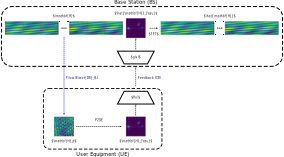
\includegraphics[width=\linewidth]{./images/00_downlink_p2d_feedback_horiz_diag.png}
    % \input{figure/csinet_quant.pdf_tex}
    \caption{Compressive CSI estimation based on linear P2D estimator. First,
    we use downlink pilots to 
    generate a sparse, frequency domain CSI
    estimate 
    of size $M_f << N_f$. We then apply
    the P2D estimator, $\mathbf{Q}^\dag_{N_t}$ of (\ref{eq:p2d_short}), to establish 
    the truncated
    delay domain CSI estimate.
    We train a
    learnable encoder, 
    $f(x)$,
    and decoder, $g(x)$, to compress and decode the feedback, respectively. The 
    gNB recovers
    the frequency domain
    CSI from 
    the decoded 
    delay domain CSI estimate.}
    \label{fig:p2d}
\end{figure}

\section{Pilots-to-delay Estimator (P2DE)}

Denote $\boldeta_i \in \mathbb{C}^{N_f}$ as the $i$-th row of the spatial-frequency matrix $\mathbf{H}$, and denote the downsampled version of $\boldeta_i$ as $\boldeta_{d,i} \in \mathbb{C}^{M_f}$ where $M_f << N_f$. Thus, the spatial-frequency CSI, $\mathbf{H}$, and its downsampled counterpart, $\mathbf{H}_d$, can be written as,
\begin{equation}
	\mathbf{H} = \begin{bmatrix} \boldeta_1 \\ \boldeta_2 \\ \vdots \\ \boldeta_{N_b} \\\end{bmatrix}\in\mathbb{C}^{N_b \times N_f}, \; \mathbf{H}_d = \begin{bmatrix} \boldeta_{d,1} \\ \boldeta_{d,2} \\ \vdots \\ \boldeta_{d,N_b} \\\end{bmatrix}\in\mathbb{C}^{N_b \times M_f}.
\end{equation}
$\boldeta_{d,i}$ is related to $\boldeta_i$ by the downsampling matrix for the $i$-th antenna port, $\mathbf{P}_i$, as
\begin{equation}
	\boldeta_{d,i} = \boldeta_i \mathbf{P}_i \; \forall \; i \in [1, \dots, N_b].
\end{equation}
Denote the delay-domain CSI vector, $\tilde{\boldeta}_i$, which is defined as
\begin{equation}
	\tilde{\boldeta}_{i}\mathbf{F} = \boldeta_i, \label{eq:dft}
\end{equation}
where $\mathbf{F}$ is the $\mathbf{C}^{N_f \times N_f}$ discrete Fourier transform (DFT) matrix. To relate the frequency domain pilots to the delay domain, we apply the pilot downsampling matrix $\mathbf{P}_i$ to both sides of \ref{eq:dft},
\begin{align}
	\tilde{\boldeta}_{i}\mathbf{F}\mathbf{P}_i = \boldeta_i\mathbf{P}_i \nonumber \\
	\tilde{\boldeta}_{i}\mathbf{Q}_i = \boldeta_{d,i} \label{eq:qmat}
\end{align}
where $\mathbf{Q}_i=\mathbf{F}\mathbf{P}_i\in\mathbb{C}^{N_f\times M_f}$ is the downsampled DFT matrix.
Leveraging the sparsity of CSI data in the delay domain (see Section~\ref{sect:sparse-csi}, Figure~\ref{fig:freq-vs-delay}), many works choose to feedback and compress the truncated delay domain vectors, $\tilde{\boldeta}_{c,i}\in\mathbb{C}^{N_t}$. The zero-padded vector $\tilde{\boldeta}_{i}$ defined as
\begin{align} 
	\tilde{\boldeta}_{i} = \left[\tilde{\boldeta}_{c,i}, \mathbf{0}_{N_f - N_t}\right]. \label{eq:p2d_short}
\end{align}

Based on \ref{eq:qmat}, the delay domain can be related directly to the pilots by taking the pseudoinverse,
\begin{align}
	\tilde{\boldeta}_{i}\mathbf{Q}_i\mathbf{Q}_i^T &= \boldeta_{d,i}\mathbf{Q}_i^T \nonumber \\
	\tilde{\boldeta}_{i} &= \boldeta_{d,i}\mathbf{Q}_i^T\left(\mathbf{Q}_i\mathbf{Q}_i^T\right)^{-1} \nonumber \\
	&= \boldeta_{d,i}\mathbf{Q}_i^{\#} \label{eq:p2d}
\end{align}

\subsection{Regularization of P2DE} \label{sec:odir}

When the pilot patterns $\mathbf{P}_i$ are equidistant and regularly spaced, the P2DE matrices $\mathbf{Q}_i\mathbf{Q}_i^T$ are typically well-conditioned. However, more irregular patterns can result in ill-conditioned matrices $\mathbf{Q}_i\mathbf{Q}_i^T$, making these matrix inversion unstable.

To compensate for this ill-conditioning, we propose to use off-diagonal regularization (ODIR) to condition the P2DE matrices. Denote $\mathbf{R} = \mathbf{Q}_i\mathbf{Q}_i^T$ and $R_{ij}$ as the element in the $i$-th row and $j$-th column of the matrix. We select a non-negative real scaling factor $\delta \in \mathbb{R}^{+}$ to scale down the off-diagonal elements of $\mathbf{R}$. The element of the resulting ODIR matrix, $\mathbf{R}_{\text{ODIR}}$, are written as
\begin{align}
    R_{ij, \text{ODIR}} &= 
        \begin{cases}
            R_{ij} & \text{if } i = j\\
            \frac{R_{ij}}{1+\delta} & \text{if } i \neq j.
        \end{cases}
\end{align}

\begin{figure}[!hbtp]
    \centering
    \includegraphics[width=\linewidth]{images/01_p2d_pilots_diag_with_resource_grid.png}
    \caption{(a) LTE Resource Blocks and CSI-RS locations where antenna port pilots are allocated. (b) Schematic for diagonal pilots with relevant parameters, size of diagonal $D$ and frequency downsampling ratio $\text{DR}_f$. In this diagram, $N_b=32, D=4, \text{DR}_f=\frac 18$. The pilot matrix $\mathbf{P}_j$ indicates the downsampling pattern for the $j$-th element of the diagonal pattern. The number of subframes necessary to populate (b) is inversely proportional to $D$.}
    \label{fig:p2d_diag}
\end{figure}

\subsection{Diagonal Pilot Allocations for 3GPP Standards}


3GPP specifications describe the allocation of pilots to time-frequency resources in 4G/LTE \cite{ref:3gpp.36.211, ref:Asplund2020} and 5G/NR \cite{ref:3GPPTS38.211V15.8.0} radio networks. In LTE, the resource elements reserved for downlink pilot estimation are called CSI reference signals (CSI-RS), while in NR, the analogous resource elements are called demodulation reference signals (DMRS). 

\begin{figure}[!hbtp]
    \centering
    \includegraphics[width=\linewidth]{images/03_p2d_pilots_diag_with_resource_grid_5gnr_ortho.png}
    \caption{(a) 5G NR Resource Blocks and DMRS locations where antenna port pilots are allocated. (b) Schematic for diagonal pilots with relevant parameters, size of diagonal $D$ and frequency downsampling ratio $\text{DR}_f$. In this diagram, $N_b=32, D=4, \text{DR}_f=\frac 18$. The pilot matrix $\mathbf{P}_j$ indicates the downsampling pattern for the $j$-th element of the diagonal pattern. The number of subframes necessary to populate (b) is inversely proportional to $D$.}
    \label{fig:p2d_diag_5gnr}
\end{figure}

Algorithm~\ref{alg:p2d-diag} shows the process for acquiring the delay domain P2DE from sparse frequency domain pilots.

\begin{algorithm}
    \caption{Pilots-to-delay Estimator (P2D) for Diagonal Pilot Pattern} 
    \label{alg:p2d-diag}
    \begin{algorithmic}[1]
    \State \textbf{\emph{Input}}:
        P2DE Matrices, $\mathbf{Q}_{c,j}^\#,\;
        j\in\{1,\dots, D\}$
    \State \textbf{\emph{Input}}: Pilot spatial-frequency CSI, $\mathbf{H}_d\in\mathbb{C}^{N_b\times M_f}$
    \State \textbf{\emph{Initialize}}: Spatial-delay CSI, $\tilde{\mathbf{H}}_\tau\in\mathbb{C}^{N_b\times N_t}$
   \State \textbf{\emph{Initialize}}: Angular-delay CSI estimate, ${\mathbf{H}}_\tau
              \in\mathbb{C}^{N_b\times N_t}$
   \For {$i=1,2,\ldots, N_b$}
        \State \textbf{\# \emph{Index for $j$-th pilot matrix}}
        \State $j = ((i-1) \text{ mod } D) + 1$
        \State \textbf{\# \emph{Apply P2D to $i$-th antenna port}}
        \State ${\boldeta}_{d,i} = \mathbf{H}_d(i,:)$
        \State $\tilde{{\mathbf{H}}}_{\tau}(i,:) = {\boldeta}_{d,i}\mathbf{Q}^{\#}_{c,j}$
        \EndFor
        \State \textbf{\# \emph{Convert from spatial to angular}}
        \State ${{\mathbf{H}}}_{\tau}=\mathbf{F}_{N_b}\tilde{{\mathbf{H}}}_{\tau}$
        \State \textbf{\emph{Return}} ${{\mathbf{H}}}_{\tau}$
    \end{algorithmic} 
\end{algorithm}


\section{Heterogeneous Differential Encoding with P2DE}

Chapter~\ref{chap:markovnet} introduced the concept of differential encoding for CSI feedback compression. The delay domain P2DE CSI introduced in this Chapter can also be used in the differential encoding framework. Figure~\ref{fig:markov-p2d} showcases the data path when utilizing the P2D estimates with a differential encoding network.

\begin{figure}[!hbtp]
    \centering
    {
      \fontsize{8pt}{8pt}
      \def\svgwidth{1.0\linewidth}
      \input{./images/02_markov_ista_p2d.pdf_tex}
    }
    % \input{figure/csinet_quant.pdf_tex}
    \caption{Diagram of a CSI estimation network using compressed differential feedback based on the linear P2DE. First, downlink pilots are used to estimate a downsampled frequency domain CSI estimate, $\bar{\mathbf{H}}_t\in\mathbb{C}^{N_b \times M_f}$ where $M_f << N_f$ at the $t$-th timeslot. Then, the P2DE $\mathbf{Q}^\#_{N_t}$ of Algorithm~\ref{alg:p2d-diag} is applied to estimate $\tilde{\mathbf{H}}_t$. After P2DE, the learnable transforms $f_t(x)$ and $g_t(x)$ are used to compress and decode the feedback, respectively. For $t=1$, the encoder/decoder are applied directly to $\tilde{\mathbf{H}}_1$. In all subsequent timeslots ($t > 1$), the differential term $\mathbf{E}_t$ is compressed and fed back.}
    \label{fig:markov-p2d}
\end{figure}

To exploit the temporal correlation of the channel, 

\section{Results}

\subsection{Accuracy of P2DE}

 We assess the accuracy of the P2DE under values of $M_f$ and $D$. Fig.~\ref{fig:outdoor_p2d_init} demonstrates the accuracy of the P2DE at the UE (i.e., before compression and feedback) for different frequency downsampling ratios. The P2DE achieves impressive accuracy even under aggressive values of $\text{DR}_f$ (e.g., better than $-30$dB at $\text{DR}_f=\frac 18$). Additionally, the effect of increasing the diagonal size, $D$, is apparent at larger compression ratios (i.e., $\text{CR} \geq \frac 18$), where the accuracy of the P2DE to a value as low as $-25$dB. For smaller compression ratios (i.e., $\text{CR} \leq \frac {1}{16}$), increasing $D$ has a marginal effect on the accuracy of the P2DE.

 \begin{figure}[!hbtp]
    \centering
    \includegraphics{./images/outdoor_p2d_diag.pdf}
    \caption{P2D estimation performance under different frequency downsampling ratios ($\text{DR}_f=\frac{M_f}{N_f}$) and diagonal dimensions ($D$) for the Outdoor COST2100 dataset. Downsampling is done along the frequency axis.}
    \label{fig:outdoor_p2d_init}
\end{figure}

We assess the accuracy of the P2DE assuming noise from pilot estimation. To simulate pilot estimation error, we use additive Gaussian noise,
\begin{align*}
    \hat{\mathbf{H}}_d &= \mathbf{H}_d + \mathbf{N}_d
\end{align*}
where the elements of $\mathbf{N}_d$, $\mathbf{N}_d(i,j) \sim \mathcal{N}(0, \sigma^2)$ for $i \in \left[1,2,\dots, N_b\right], j \in \left[1,2,\dots, M_f\right]$. To achieve different SNR values for $\hat{\mathbf{H}}_d$, we simply vary the noise variance $\sigma^2$, and we use the P2DE at different pilot estimation noise levels. Figure~\ref{fig:snr_sweep} shows the accuracy of the P2DE for different values of $\sigma^2$.

In addition to varying the pilots estimation SNR, we also showcase the effect of varying $\delta$ (i.e., the ODIR parameter as described in Section~\ref{sec:odir}). We observe that $\delta$ helps the P2DE achieve better performance under both low-noise and noisy conditions, i.e.,

\begin{itemize}
    \item \textbf{Low-noise condition (SNR $\mathbf{=-20}$ dB)}: The P2DE goes from $-8$ dB to $-22$ dB for $\delta=0$ and $\delta=0.5$, respectively.
    \item \textbf{Noisy condition (SNR $\mathbf{\geq -10}$ dB)}: The P2DE goes from $-9$ dB to $-30$ dB for $\delta=0$ and $\delta=0.5$, respectively.
\end{itemize}

\begin{figure}[!hbtp]
    \centering
    \includegraphics{outdoor_snr_sweep_delta_D4_sz32.pdf}
    \caption{Accuracy of P2DE output, $\mathbf{H}_{\tau}$, assuming noisy pilots, $\hat{\mathbf{H}}_d$. Additive Gaussian noise is used to model the error inherent in pilot estimation. Here, $D=4, \text{DR}_f=\frac{1}{32}$.}
    \label{fig:snr_sweep}
\end{figure}

\subsection{P2DE Compression Network Comparison}

Having assessed the initial accuracy of the P2DE at the UE, we now apply a deep learning network to compress the output of the P2DE. Figure~\ref{fig:outdoor_drcr_sweep} demonstrates the accuracy of ISTANet+ \cite{ref:zhang2018ista} for multiple compression ratios (CR) using the P2DE as its input. For progressively smaller compression ratios, the accuracy of ISTANet+ remains stable until $\text{DR}_f=\frac{1}{32}$, at which point the network's performance degrades.

\begin{figure}[!hbtp]
    \centering
    \includegraphics{./images/outdoor_drcr_D_sweep.pdf}
    \caption{Performance of ISTANet+ for multiple compression ratios using P2D estimates with different downsampling ratios ($\text{DR}_f=\frac{M_f}{N_f}$) for the Outdoor COST2100 dataset. Non-diagonal pattern ($D=1$) is compared with a diagonal pattern of size $D=4$. Performance for $\text{DR}_f=1/1$, $D=4$ is omitted since it is equivalent to the $\text{DR}_f=1, D=1$ case.}
    \label{fig:outdoor_drcr_sweep}
\end{figure}

In addition to ISTANet+, we assess the accuracy deep CNN autoencoders using P2DE as an input. Figure~\ref{fig:outdoor_net_ablation} shows the accuracy of ISTANet+ compared to ENet \cite{ref:Sun2021ENet} and SphNet \cite{ref:liu2020sphnet}. The performance of ISTANet+ is better than both ENet and SphNet at larger compression ratios ($\text{CR}\in [\frac 14, \frac 18]$), and the performance of ISTANet+ and ENet is comparable at $\text{CR}=\frac {1}{16}$.

\begin{figure}[!hbtp]
    \centering
    \includegraphics{outdoor_net_compare.pdf}
    \caption{Performance comparison for different feedback compression networks using P2D estimates ($\text{DF}_f=1/16, D=4$) for Outdoor COST2100 dataset. For all tested networks, we use $N_{\text{phase}}=4$, resulting in an augmented training set with $80$k samples.}
    \label{fig:outdoor_net_ablation}
\end{figure}

To assess the accuracy of these networks under quantization, we also conduct an experiment where the latent feedback elements are subjected to $\mu$-law companding and uniform quantization (as described in Section~\ref{sec:markov-results}). We present these results in Figure~\ref{fig:net_quant}.

\begin{figure}[!hbtp]
    \centering
    \includegraphics[width=\linewidth]{./images/outdoor_net_quant.pdf}
    \caption{Tested networks where feedback is subject to $\mu$-law companding ($\mu=255$) and uniform quantization for different numbers of quantization bits. P2DE parameters are $D=4, \text{DR}_f=\frac{1}{16}$.}
    \label{fig:net_quant}
\end{figure}
\chapter{Conclusion} \label{chap:conclusion}

This thesis surveyed techniques to improve the performance and efficiency of deep neural networks for the task of MIMO CSI estimation. In Chapter~\ref{chap:sph_norm} we discussed the importance of data pre-processing techniques, and we showed the efficacy of our proposed spherical normalization technique. In Chapter~\ref{chap:markovnet}, we exploited the temporal correlation of the wireless channel, and we demonstrated the superior performance and efficiency of a deep differential encoder compared to recurrent neural networks. Finally, in Chapter~\ref{chap:p2d}, we presented two main contributions: an accurate estimator of the delay domain CSI based on sparse frequency domain pilots and a hetergeneous differential encoding network combining deep compressed sensing networks with autoencoders. We showed the accuracy of our pilot-based delay domain estimator, even under aggressive sparsity and noisy pilot estimates. Furthermore, we verified the improved performance of heterogeneous networks over homogeneous networks.
\chapter{Conclusion} \label{chap:conclusion}

This dissertation investigates techniques to improve the performance and efficiency of deep neural networks for the task of MIMO CSI estimation. In Chapter~\ref{chap:sph_norm} we discussed the importance of data pre-processing techniques, and we showed the efficacy of our proposed spherical normalization technique. In Chapter~\ref{chap:markovnet}, we exploited the temporal correlation of the wireless channel, and we demonstrated the superior performance and efficiency of a deep differential encoder compared to recurrent neural networks. In Chapter~\ref{chap:p2d}, we presented two main contributions: an accurate estimator of the delay domain CSI based on sparse frequency domain pilots and a hetergeneous differential encoding network combining deep compressive sensing networks with autoencoders. We showed the accuracy of our pilot-based delay domain estimator, even under aggressive sparsity and noisy pilot estimates. Furthermore, we verified the improved performance of heterogeneous networks over homogeneous networks. Finally in Chapter~\ref{chap:comp-effic}, we proposed a scheme which re-uses a simple model on contiguous blocks of multiple subcarriers, and we showed that this method can maintain accuracy while reducing the computational complexity of the network by a factor of 10.  

Across all these works, we investigated techniques which exploited domain knowledge of the wireless channel to improve estimation accuracy and computational efficiency while better conforming to 3GPP protocols. Further work in CSI compression should take a similar approach by taking advantage of features of the wireless channel, the communications protocol, or CSI data itself.

\section{Future Works}

In addition to the work discussed in this dissertation, there are important additional directions which future works in deep learning for CSI compression should address. Here, we discuss a few such directions, including compression bounds for CSI estimation and networks with trainable codewords.

\subsection{Rate-distortion Bounds for CSI Feedback}

Many works provide results for their proposed CSI feedback networks using the NMSE at a small number of compression ratios. This approach allows for fair comparison between comparable networks/algorithms, but it does not answer a more important question: \emph{At a given compression ratio, what is the theoretical distortion limit?}

Information theory provides us with a framework to answer this question: the rate-distortion curve. The rate-distortion of a random variable describes the optimal error that can be achieved whenever that variable is encoded using a given number of bits.

The challenge with applying rate-distortion theory to MIMO CSI data is the lack of well-defined distributions for practical channel data. While rate-distortion bounds are known for well-defined distributions (e.g., univariate or multivariate Gaussian distributions), the same can not be said for empirical data.

One possible approach to constructing a rate-distortion curve is to estimate the differential entropy of quantized CSI data. For a CSI matrix, $\mathbf{H}$, assume i.i.d. $\mathbf H_{(i,j)}$ where $i$ ($j$) denotes the row (column) of $\mathbf{H}$. The differential entropy of the $(i,j)$-th element is
\begin{align*}
	h(\mathbf H_{(i,j)}) &= - \int p(\mathbf H{(i,j)} = k) \log p(\mathbf H_{(i,j)} = k) dk,
\end{align*}
In practice, the distribution $p(\mathbf H_{(i,j)})$ is difficult to obtain. We can instead resort to the Kozachenko–Leonenko (KL) estimator \cite{ref:Kozachenko1987SampleEstimate} for each element in $\mathbf H$ and average over the elements,
\begin{align}
	h(\mathbf H) &\leq \sum_{i}^{R_d}\sum_{j}^{n_T} \hat h(\mathbf H_{(i,j)}) = h_{\text{UB}}(\mathbf H), \label{eq:csi-diff-ent}
\end{align}
for KL estimator $\hat h$. Based on Theorem 8.3.1 from Cover \cite{ref:Cover1999Elements}, for sufficiently small quantization interval $\Delta = \frac {1}{2^n}$, the entropy of a quantized random variable is related to its differential entropy as,
\begin{align}
  H(\mathbf H^{\Delta}) &= h(\mathbf H) + n, \label{eq:cover-thm}
\end{align}
for $n$-bit quantization. Thus, the differential entropy estimator admits an estimate for the entropy of the quantized CSI, $\hat H({\mathbf H}^\Delta) = \hat h(\mathbf H) + n$.

To establish a rate-distortion curve, we can use the estimator outlined above on CSI data with Gaussian noise, i.e.
\begin{align*}
	\mathbf H_{\sigma,(i,j)} &= \mathbf H_{(i,j)} + v \text{ for i.i.d } v \sim \mathcal{N}(0,\sigma^2).
\end{align*}
Using the corrupted CSI matrices $\mathbf H_{\sigma}=\left[\mathbf H_{\sigma,(i,j)}\right]_{i\in [R_d],j\in [N_b]}$, we calculate the bounds $\hat h(\mathbf H_{\sigma}^\Delta)$ from or (\ref{eq:csi-diff-ent}) for different noise levels $\sigma$ to establish a rate-distortion curve.

\subsection{Trainable Codewords}

In addition to estimating the rate-distortion bounds of CSI data, new works should investigate techniques for improving the compression efficiency of CSI feedback networks. Some prior work has investigated feedback quantization in deep learning-based CSI compression. In \cite{ref:Yang2019DeepCMC}, the authors propose DeepCMC, an autoencoder structure where the continuous compressed elements are discretized via uniform quantization then encoded using context adaptive binary arithmetic coding (CABAC) \cite{ref:Marpe2003CABAC}. Since uniform quantization is non-differentiable, the authors do not perform true quantization during training and instead apply uniformly distributed noise to approximate quantization noise \cite{ref:Yang2019DeepCMC}. In \cite{ref:Mashhadi2020AnalogDeepCMC}, the authors propose AnalogDeepCMC, which encodes latent elements as power-normalized complex elements and decodes using maximal ratio combining. The authors also report the achieved rate of AnalogDeepCMC for different CSI overhead ratios.

Further work into trainable codewords might borrow ideas from deep learning based image compression. For example, the soft-to-hard vector quantization (SHVQ) framework \cite{ref:Agustsson2017SoftToHard} could be used to imbue a CSI compression network with quantized codewords. To describe the framework, we choose a vector dimension, $d$, by which to partition the latent space $\mathbf Z = f_e(\mathbf H, \theta_e)$, and we denote the vectorized version of $\mathbf Z \in \mathbb R^{r}$ as $\tilde{\mathbf Z} \in \mathbb R^{r/d \times d}$. We define the $d$-dimensional codebook of size $L$ as $\mathbf C \in \mathbb R^{d\times L}$. The soft assignments of the $j$-th latent vector $\tilde{\mathbf z}_j$ can be written as
\begin{align}
\phi(\tilde{\mathbf z}_j) &= \left[\frac{\text{exp}(-\sigma \Arrowvert \tilde{\mathbf z}_j - \mathbf c_\ell\Arrowvert^2)}{\sum_{i=1}^L\text{exp}(-\sigma \Arrowvert \tilde{\mathbf z}_j - \mathbf c_i\Arrowvert^2)}\right]_{\ell\in [L]} \in \mathbb R^L \label{eq:soft_assign}
\end{align}
where (\ref{eq:soft_assign}) is typically referred to as the \emph{softmax} function, a differentiable alternative to the max function. The hyperparameter $\sigma$ controls the temperature of the softmax scores, with a lower $\sigma$ yielding a more uniform distribution and a higher $\sigma$ yielding a ``peakier'' distribution (i.e., as $\sigma \to \infty \Rightarrow \phi(\tilde z_j) \to $ a one-hot vector). Using the soft assignments, the latent vectors are quantized based on the codebook $\mathbf C \in \mathbb R^{d \times L}$,
\begin{align}
Q(\tilde{\mathbf z}_j,\mathbf C) &= \phi(\tilde{\mathbf z}_j) \mathbf C^T. \label{eq:soft_quant}
\end{align}
where we refer the $Q(\tilde{\mathbf z}_j, \mathbf C)$ as the `SoftQuantize' function. When applying $Q(\cdot)$ to the $r/d$ rows of $\tilde{\mathbf Z}$, we write the SoftQuantize function as a matrix operation, $\mathbf Q(\tilde{\mathbf Z},\mathbf C) \in \mathbb R^{r/d \times d}$. The matrix of soft-quantized latent vectors is then reshaped into the original latent vector dimension, $\hat{\mathbf Z} \in \mathbb R^r$, and the decoder produces the CSI estimates as $\hat{\mathbf H} = h(\hat{\mathbf Z}, \mathbf C)$. An abstract illustration of an autoencoder using soft quantization can be seen in Figure~\ref{fig:csinet_quant}.

\begin{figure*}[!hbtp]
\centering
\def\svgwidth{0.8\linewidth}
\input{images/csinet_quant.pdf_tex}
\caption{Abstract architecture for a CSI compression network with the `SoftQuantize' layer ($Q(\tilde{\mathbf Z})$), a continuous, softmax-based relaxation of a $d$-dimensional quantization of the latent layer $\mathbf Z$.}
\label{fig:csinet_quant}
\end{figure*}

To optimize the network with soft quantization, the loss function can be made to resemble the canonical rate-distortion function by adding an entropy penalization term,
\begin{align}
\underset{\theta_e, \theta_d, \mathbf C}{\text{argmin}}\; \frac 1N &\sum_{i=1}^N\Arrowvert \mathbf H_i - g(Q(f(\mathbf H_i, \theta_e), \mathbf C), \theta_d) \Arrowvert^2 \nonumber \\
&+ \lambda \left(\Arrowvert\theta_e\Arrowvert^2+\Arrowvert\theta_d\Arrowvert^2+\Arrowvert \mathbf C \Arrowvert^2\right) \label{eq:loss_entropy} \\
&+ m\beta H(\phi), \nonumber
\end{align}
where $H(\phi)=H(p,q)$ is the crossentropy based on the hard and soft probability estimates $p$ and $q$, respectively. Before defining the estimates $p$ and $q$, we briefly discuss the population probabilities of the latent codewords. Denote the symbol encoder/decoder pair as $E:\mathbb R^d \to [L]^d$/$D:[L]^d \to \mathbb R^d$. Denote the distribution of latent variables as $\mathsf Z$ such that $\mathbf z \sim \mathsf Z$ with the encoder $E(\mathsf Z)=\mathbf e$ . The entropy of $\mathsf Z$ is given as 
\begin{align*}
H(E(\mathsf Z)) &= -\sum_{\mathbf e\in[L]^d}P(E(\mathsf Z) = \mathbf e)\log_2(P(E(\mathsf Z)=\mathbf e)).
\end{align*}
In practice, the true population probabilities $P(E(\mathsf Z))$ are inaccessible, and we must estimate the probability masses via finite sampling over the encoder's outputs, $e(\mathbf z)$. The hard probability estimate $p_j$ of the $j$-th codeword is
\begin{align*}
p_j &= \frac{|\{e_l(\mathbf z_i)|l\in[d], i \in [N], e_l(\mathbf z_i)=j\}|}{dN}.
\end{align*}
The soft assignments of $\phi$ admit valid probability masses, $q_j = \phi(\tilde{\mathbf z})$, over the codewords. Using histogram estimates $p_j$ and the soft assignments $q_j$, the crossentropy term is written
\begin{align*}
H(\phi) := H(p,q) &= -\sum_{j=1}^L p_j\log q_j = H(p) + D_{\text{KL}}(p\Arrowvert q)
\end{align*}
where $D_{\text{KL}}(p\Arrowvert q)=-\sum_{j=1}^L p_j \log\left(\frac{p_j}{q_j}\right)$ is the Kullback-Liebler (KL) divergence. Due to the nonnegativity of $D_{\text{KL}}$, $H(\phi)$ is an upper bound on $H(p)$, and so (\ref{eq:loss_entropy}) is a valid optimization target.

% \chapter{Conclusions}
\label{chap:conclusion}

We have explored non-convex optimization in the context of wireless communications under geometrical perspectives, using new techniques developed for seemingly unrelated problems. We have also proposed new geometrical perspectives for both grant-free access and grant-free scheduling, leveraging the underlying properties of the computational space to improve the performance of these tasks with reasonable computational complexity and minimal ad-hoc settings.

% WF-CMA
\section{CMA via Wirtinger Flow}
First, we used known results and algorithms for phase retrieval and applied this knowledge into the blind beamforming problem. We generalized the convergence analysis of WF for our WF-CMA algorithm by incorporating new conditions of subgaussian signal sources and average modulus, demonstrating its global convergence for blind signal recovery with high probability under limited data samples. 
We characterized the local geometry of the CM cost function in terms of smoothness and convexity, which enables parameter updates to remain within the basin of attraction for a defined stepsize. This allows to establish a more aggressive stepsize than the traditional gradient-descent CMA approaches, tackling the slow convergence of the latter with no significant increase in the computational cost.  


% RMSR
\section{Riemannian Multiple Signal Recovery}
We also developed a Riemannian framework for blind source recovery problems, and to the best of our knowledge, is the first work using these techniques for CMA-based formulations.
This is achieved by means of minimizing a CMA cost function, such that the orthogonality of different demixers is embedded in the geometry of a Riemannian manifold. We derive this geometry and obtain the geometrical definitions that allow to minimize over the manifold as the search space of the optimization problem. The results of our approach show high probability of successful recovery of all sources with a reasonable number of samples, for rather large system sizes and different modulation schemes. 


% U-SCH
\section{Unsupervised Riemannian User Scheduling}
Last but not least, we focused on the uplink user scheduling problem that exploits spatial multiplexing in MIMO systems. To mitigate the intra-group interference, instead of directly scheduling users with high channel dissimilarity, we developed a general uplink user scheduling strategy that selects users from different high-similarity channel clusters, by exploiting unsupervised learning algorithms without the requirement of a significant number of labeled data. We identified a Riemannian manifold that inherently describes the similarity of channels with respect to their cross-correlation, which is invariant to both phase and magnitude differences. Using this manifold as the underlying computational space, we exploit the retrieved similarity information to assist in the scheduling of users.
Under a variety of performance metrics to evaluate user scheduling, simulations indicate that the combination of a learning-enabled channel clustering can exploit the spatial compatibility effectively to reduce inter-group interference when compared with other benchmarks. 




\cleardoublepage
\phantomsection
%\addcontentsline{toc}{section}{References}
\addcontentsline{toc}{chapter}{References}
\bibliographystyle{IEEEtran}
\bibliography{cited_works}

\singlespacing
\appendix
\chapter{Computational Complexity of Common Layers}
\label{appdx:complexity}
Based on the measures of computational complexity in Chapter~\ref{chap:sph_norm} Section~\ref{sect:dl_overview}, i.e. FLOPs and parameters, we provide the corresponding formulas for common layers and operations used in the networks described in this thesis. Note that any arithmetic operation (e.g., addition, multiplication) or non-linearity consumes a single FLOP, and certain non-linearities require a single parameter (e.g., the negative slope of a Leaky ReLU).

\section{Linear Layer} \label{appdx:complexity-linear}
Denote parameter matrix $\mathbf{A}\in\mathbb{R}^{M\times N}$ and the input vector $\mathbf{b}\in\mathbb{R}^{N}$. The output of a linear layer, $\mathbf{o}\in\mathbb{R}^M$, is given as
\begin{align*}
	\mathbf{o} &= \mathbf{A}\mathbf{b}.
\end{align*}
If the linear layer contains a bias term, then an additional column $\mathbf{a}_0$ is appended to the end of the matrix $\mathbf{A}$ as
\begin{align*}
	\mathbf{A}_{\text{bias}} &= \begin{bmatrix}\mathbf{A} & \mathbf{a}_0\end{bmatrix},
\end{align*}
and correspondingly, the input vector is padded with a single one,
\begin{align*}
	\mathbf{b}_{\text{bias}} &= \begin{bmatrix}\mathbf{b} & 1\end{bmatrix}.
\end{align*}

\textbf{FLOPs}: A linear layer has the same number of FLOPs as a matrix-vector multiplication, i.e.
\begin{align*}
	\text{FLOPs}_{\text{linear}} &= M(N-1)
\end{align*}

\textbf{Parameters}: The size of the matrix $\mathbf{A}$ determines the number of parameters in the layer, i.e.,
\begin{align*}
	P_{\text{linear}} &= MN
\end{align*}

\section{Convolutional Layer}

In a convolutional layer, the complexity is driven by the number of kernels ($N_k$), the height/width of kernel ($H_k/W_k$), and the channels/height/width of the input data ($C/H/W$). Denote the input data as $\mathbf I\in\mathbb{R}^{C\times H\times W}$, the kernel as $\mathbf{K}\in\mathbb{R}^{N_k\times H_k\times W_k}$, and the output image as $\mathbf O\in\mathbb{R}^{N_k\times H\times W}$. The convolution operation assigns a value to each element of the output using the following equation,
\begin{align}
	\mathbf{O}(i,j,k) &= \sum_{c=1}^{C}\sum_{h=1}^{H_k}\sum_{w=1}^{W_k} K(i,j+h,k+w)I\left(c,j+h-\left\lfloor\frac{H}{2}\right\rfloor,k+w-\left\lfloor\frac{W}{2}\right\rfloor\right)
\end{align}
Whenever the height or width indices of $\mathbf{I}$ are out of the range $[1,\dots,H]$ or $[1,\dots,W]$, the elements involved in the convolution are determined by the padding (e.g., zero padding, reflected padding, etc.).

\textbf{FLOPs}: The number of FLOPs in a convolutional layer is given by the following formula,
\begin{align*}
	\text{FLOPs}_{\text{conv}} &= C\times H \times W \times N_k \times H_k \times W_k
\end{align*}

\textbf{Parameters}: The number of parameters in a convolutional layer is given by the following formula,
\begin{align*}
	P_{\text{conv}} &= N_k\times H_k\times W_k
\end{align*}

\section{Soft Threshold Function}

The soft threshold function used in ISTANet+ \cite{ref:zhang2018ista} is given in (\ref{eq:soft}), replicated below as,
\begin{align*}
    \text{soft}(x, \theta) &= \text{sign}(x)\text{ReLU}(|x|-\theta),
\end{align*}
where $\theta$ is the threshold function.

\textbf{FLOPs}: We consider a single soft threshold to consume one FLOP.

\textbf{Parameters}: The soft threshold function requires one parameter to be stored, $\theta$.
\chapter{Autoregressive Markov Models}
\label{appdx:autoregressive}

In Chapter~\ref{chap:markovnet} Section~\ref{sect:diff-enc}, we introduced a differential encoding network based on an autoregressive Markov model that was A) one-step and B) scalar. In this appendix, we show how we can generalize both the number of steps and the dimension of the Markov model.

Recall the truncated delay domain CSI at the $t$-th timeslot, $\mathbf{H}_{t}\in\mathbb{C}^{R_d \times N_b}$. Rather than the one-step, scalar model $\hat\gamma \in \mathbb R^+$ (see (\ref{eq:diff-estim}) in Section~\ref{sect:diff-enc}), we can derive a $p$-step, multivariate predictor. A $p$-step autoregressive model for $\mathbf{H}_t$ can be written generally as a function of $p$ previous timeslots,
\begin{align*}
	\hat{\mathbf{H}}_t &= f(\mathbf{H}_{t-1}, \mathbf{H}_{t-2}, \dots, \mathbf{H}_{t-p}).
\end{align*}
Given $p$ prior CSI samples, the mean-square optimal predictor $\hat{\mathbf{H}}_t$ is a linear combination of these the prior CSI samples,
\begin{equation}
\mathbf{\hat H}_{t} = \mathbf{H}_{t-1} \mathbf W_{1} + \dots + \mathbf{H}_{t-p} \mathbf W_{p} + \mathbf E_t.
\end{equation}

Where $\mathbf{W}_{i}$ is the coefficient matrix foro the $i$-th timeslot with dimension $\mathbb{C}^{N_b \times N_b}$, and $\mathbf{E}_t$ is the error term at time $t$, which is uncorrelated with the CSI samples (i.e. $\mathbf H_{t-i}^H \mathbf E_t = 0$ for all $i \in [0, \dots, p]$). To solve for the matrices $\mathbf{W}_{t-1}, \dots, \mathbf{W}_{t-p}$, we first pre-multiply by $\mathbf H_{t-i}^H$,
\begin{align}
\mathbf{H}_{t-i}^H\mathbf{\hat H}_{t} &= \mathbf{H}_{t-i}^H\mathbf{H}_{t-1} \mathbf W_{1} + \dots + \mathbf{H}_{t-i}^H\mathbf{H}_{t-p} \mathbf W_{p} + \mathbf{H}_{t-i}^H\mathbf E_t \nonumber \\
                    &= \mathbf{H}_{t-i}^H\mathbf{H}_{t-1} \mathbf W_{1} + \dots + \mathbf{H}_{t-i}^H\mathbf{H}_{t-p} \mathbf W_{p}. \label{eq:var-init}
\end{align}

Denote the correlation matrix 
$\mathbf R_i = \mathbb E [\mathbf H^H_{t-i}\mathbf H_{t}]$. If temporal coherence between timeslots is maintained, then we may assume that CSI matrices arise from a stationary process, implying the following properties:
\begin{enumerate}
  \item $\mathbf R_i = \mathbb E [\mathbf H^H_{t-i}\mathbf H_{t}] = \mathbb E [\mathbf H^H_{t}\mathbf H_{t+i}]$
  \item $\mathbf R_i = \mathbf R^H_{-i}$
\end{enumerate}

With these properties in mind, we take the expectation of (\ref{eq:var-init}), 
resulting in a linear combination of $\mathbf R_i$ matrices,
\begin{align*}
\mathbb E\left[\mathbf{H}_{t-i}^H\mathbf{\hat H}_{t}\right] &= \mathbb E\left[\mathbf{H}_{t-i}^H\mathbf{H}_{t-1} \mathbf W_{1}\right] + \dots + \mathbb E\left[\mathbf{H}_{t-i}^H\mathbf{H}_{t-p} \mathbf W_{p}\right] \\
\mathbf R_{i+1} &= \mathbf{R}_{i} \mathbf W_{1} + \dots + \mathbf{R}_{i-p+1} \mathbf W_{p}. 
\end{align*}
For $p$ CSI samples (i.e., for $i \in [0, 1, \dots, p-1]$), we write a system of $p$ equations, admitting the following,
\begin{align}
  \begin{bmatrix}
    \mathbf R_{1} \\ \mathbf R_{2} \\ \dots \\ \mathbf R_{p} \\
  \end{bmatrix}
  &= 
  \begin{bmatrix}
    \mathbf R_{0} & \mathbf R_1^H & \dots  & \mathbf R_{p-1}^H \\
    \mathbf R_{1} & \mathbf R_0   & \dots  & \mathbf R_{p-2}^H \\
    \vdots      &         & \ddots & \vdots \\
    \mathbf R_{p-1} & \mathbf R_{p-2}   & \dots  & \mathbf R_{0} \\
  \end{bmatrix}
  \begin{bmatrix}
    \mathbf W_{1} \\ \mathbf W_{2} \\ \dots \\ \mathbf W_{p} \\
  \end{bmatrix}. \label{eq:toep}
\end{align}
Finally, we solve for the coefficient matrices by inverting the Toeplitz matrix,
\begin{align}
  \begin{bmatrix}
    \mathbf W_{1} \\ \mathbf W_{2} \\ \dots \\ \mathbf W_{p} \\
  \end{bmatrix}
  &= 
  \begin{bmatrix}
    \mathbf R_{0} & \mathbf R_1^H & \dots  & \mathbf R_{p-1}^H \\
    \mathbf R_{1} & \mathbf R_0   & \dots  & \mathbf R_{p-2}^H \\
    \vdots      &         & \ddots & \vdots \\
    \mathbf R_{p-1} & \mathbf R_{p-2}   & \dots  & \mathbf R_{0} \\
  \end{bmatrix}^{-1}
  \begin{bmatrix}
    \mathbf R_{1} \\ \mathbf R_{2} \\ \dots \\ \mathbf R_{p} \\
  \end{bmatrix}. \label{eq:toep-sol}
\end{align}
Thus, the solution to multi-step, multivariate Markov model is a function of the correlation matrices.

Since the distributions of $\mathbf{H}_i$ are not known, we cannot calculate the expectations in the correlation matrices, $\mathbf R_i$. Instead, we estimate the sample correlation matrices with the training data, i.e.,
\begin{align*}
	\hat{\mathbf{R}}_i = \frac{1}{N_{\text{train}}} \sum_{j}^{N_{\text{train}}} \mathbf{H}_{t-i}(j)^{H}\mathbf{H}_{t}(j),
\end{align*}
where $j$ indexes over the training data. Now, we write the estimators, $\hat{\mathbf{W}}_i$, with respect to the sample correlation matrices,
\begin{align}
  \begin{bmatrix}
    \hat{\mathbf W}_{1} \\ \hat{\mathbf W}_{2} \\ \dots \\ \hat{\mathbf W}_{p} \\
  \end{bmatrix}
  &= 
  \begin{bmatrix}
    \hat{\mathbf R}_{0} & \hat{\mathbf R}_1^H & \dots  & \hat{\mathbf R}_{p-1}^H \\
    \hat{\mathbf R}_{1} & \hat{\mathbf R}_0   & \dots  & \hat{\mathbf R}_{p-2}^H \\
    \vdots      &         & \ddots & \vdots \\
    \hat{\mathbf R}_{p-1} & \hat{\mathbf R}_{p-2}   & \dots  & \hat{\mathbf R}_{0} \\
  \end{bmatrix}^{-1}
  \begin{bmatrix}
    \hat{\mathbf R}_{1} \\ \hat{\mathbf R}_{2} \\ \dots \\ \hat{\mathbf R}_{p} \\
  \end{bmatrix}. \label{eq:toep-sol-est}
\end{align}

If a more simple model is desired, then we can construct scalar estimators for each timeslot. Denote the mean of all elements in the correlation matrix as,
\begin{align*}
  r_i = \mathbb{E}\left[\sum_{k}^{R_d} \sum_{\ell}^{N_b}\mathbf{R}_i^{(k,\ell)}\right]
\end{align*}
where $\mathbf{R}_i^{(k, \ell)}$ is the element from the $k$-th row and $\ell$-th column of $\mathbf{R}_i$. The resulting system of equations for scalar model is given as
\begin{align}
  \begin{bmatrix}
    \gamma_{1} \\ \gamma_{2} \\ \dots \\ \gamma_{p} \\
  \end{bmatrix}
  &= 
  \begin{bmatrix}
    r_{0} & r_1^* & \dots  & r_{p-1}^* \\
    r_{1} & r_0   & \dots  & r_{p-2}^* \\
    \vdots      &         & \ddots & \vdots \\
    r_{p-1} & r_{p-2}   & \dots  & r_{0} \\
  \end{bmatrix}^{-1}
  \begin{bmatrix}
    r_{1} \\ r_{2} \\ \dots \\ r_{p} \\
  \end{bmatrix}. \label{eq:toep-sol-scalar}
\end{align}
Following the same logic as before, we utilize the sample versions of $\hat r_i$,
\begin{align*}
  \hat r_i &= \frac{1}{N_{\text{train}}} \sum_{j}^{N_{\text{train}}} \sum_{k}^{R_d} \sum_{\ell}^{N_b}\hat{\mathbf{R}}_i^{(k,\ell)}(j),
\end{align*}
which admits the system of equations,
\begin{align}
  \begin{bmatrix}
    \hat\gamma_{1} \\ \hat\gamma_{2} \\ \dots \\ \hat\gamma_{p} \\
  \end{bmatrix}
  &= 
  \begin{bmatrix}
    \hat r_{0} & \hat r_1^* & \dots  & \hat r_{p-1}^* \\
    \hat r_{1} & \hat r_0   & \dots  & \hat r_{p-2}^* \\
    \vdots      &         & \ddots & \vdots \\
    \hat r_{p-1} & \hat r_{p-2}   & \dots  & \hat r_{0} \\
  \end{bmatrix}^{-1}
  \begin{bmatrix}
    \hat r_{1} \\ \hat r_{2} \\ \dots \\ \hat r_{p} \\
  \end{bmatrix}. \label{eq:toep-sol-scalar-est}
\end{align}
For the one-step scalar estimator, we can derive equation (\ref{eq:gamma-hat}) from Chapter~\ref{chap:markovnet} of Section~\ref{sect:diff-enc},
\begin{align*}
  \hat{\gamma}_1 &= \frac{\hat{r}_1}{\hat{r}_0} \\
  &= \frac{\text{Trace}(\hat{\mathbf R}_1(k,l))}{\sum_k^{R_d}\sum_l^{N_b}\hat{\mathbf R}_0(k,l)}.
\end{align*}
\chapter{Matrix Regularization}
\label{appdx:odir}

In this dissertation, we encounter a few situations where we have a matrix to invert, $\mathbf{A}$, but the matrix $\mathbf{A}$ may be nearly singular. For example, in Section~\ref{sect:p2de} of Chapter~\ref{chap:p2d} we had the pseudoinverse $\mathbf{Q}_i^{\#} = \mathbf{Q}_i^T\left(\mathbf{Q}_i\mathbf{Q}_i^T\right)^{-1}$, where we would denote our matrix to invert as $\mathbf{A}=\mathbf{Q}_i\mathbf{Q}_i^T$.

As another example from Appendix~\ref{appdx:autoregressive}, we discussed the multivariate, $p$-step Markov model for CSI which was a function of the correlation matrices, $\hat{\mathbf{R}}_i$. Per equation (\ref{eq:toep-sol-est}), we denote $\mathbf{A}$ as the Toeplitz matrix populated by the $\hat{\mathbf{R}}_i$ matrices.

In either of the cases described above, the stability of the matrix inverse can be improved by regularizing the matrix. Here, we briefly describe one method for regularizing nearly singular matrices, off-diagonal regularization (ODIR).

Denote $A_{ij}$ as the element in the $i$-th row and $j$-th column of the matrix $\mathbf{A}$. We select a non-negative real scaling factor $\delta \in \mathbb{R}^{+}$ to scale down the off-diagonal elements of $\mathbf{R}$. The elements of the resulting ODIR matrix, $\mathbf{A}_{\text{ODIR}}$, are written as
\begin{align}
    A_{ij, \text{ODIR}} &= 
        \begin{cases}
            A_{ij} & \text{if } i = j\\
            \frac{A_{ij}}{1+\delta} & \text{if } i \neq j.
        \end{cases}
\end{align}
% TODO: Find the reference for ODIR. I think it was a set of lecture slides? 
\chapter{Compressed Sensing}
\label{appdx:compressed-sensing}

In Section~\ref{sect:hetero-markov} of Chapter~\ref{chap:p2d}, we introduced a heterogeneous differential encoder which utilized deep compressed sensing networks. Here, we provide a brief overview of compressed sensing algorithms.

Given a signal $\mathbf{x}\in\mathbb{R}^N$, denote a random measurement of this signal as 
\begin{align*}
    \mathbf{y} = \mathbf{\Phi}\mathbf{x}
\end{align*}
where $\mathbf{\Phi}\in\mathbb{R}^{M\times N}$ is referred to as the \emph{measurement matrix} and $\mathbf{y}\in\mathbb{R}^{M}$ is a low-dimensional measurement (i.e., $M << N$). The goal of compressed sensing is to recover the original signal $\mathbf{x}$ based on the low-dimensional measurement $\mathbf{y}$.

\end{document}